\documentclass{beamer}
\usepackage{graphicx}
\usepackage{listings}
\usepackage{amsfonts}
\usepackage{amsmath}
\usepackage{multicol}
\usepackage[pdf]{graphviz}
\usepackage[skins,breakable,listings]{tcolorbox}

\lstset{basicstyle=\ttfamily,breaklines=true}
\usepackage{upquote}
%\def\backtick{\char18}
\lstdefinestyle{backtickstyle}{literate={`}{\char}1, escapechar=@}

\usepackage{fontspec}

\makeatletter
\def\verbatim@nolig@list{}
\makeatother

\setmonofont{JetBrains Mono}[Contextuals=Alternate]

\usepackage{ocr}
\usepackage[T1]{fontenc}

\usepackage{accsupp}
\usepackage{bussproofs}
\newcommand{\noncopyable}[1]{%
\BeginAccSupp{method=escape,ActualText={}}%
#1%
\EndAccSupp{}%
}

\lstdefinelanguage{kotlin}{
comment=[l]{//},
commentstyle={\color{gray}\ttfamily},
emph={delegate, filter, firstOrNull, forEach, it, lazy, mapNotNull, println, repeat, assert, with, head, tail, len, return@},
numberstyle=\noncopyable,
emphstyle={\color{olive}},
identifierstyle=\color{black},
keywords={abstract, actual, as, as?, break, by, class, companion, continue, data, do, dynamic, else, enum, expect, false, final, for, fun, get, if, import, in, infix, interface, internal, is, null, object, open, operator, override, package, private, public, return, sealed, set, super, suspend, this, throw, true, try, catch, typealias, val, var, vararg, when, where, while, tailrec, reified, Repeat},
keywordstyle={\color{blue}\bfseries},
morecomment=[s]{/*}{*/},
morestring=[b]",
morestring=[s]{"""*}{*"""},
ndkeywords={@Deprecated, @JvmField, @JvmName, @JvmOverloads, @JvmStatic, @JvmSynthetic, Array, Byte, Double, Float, Boolean, Int, Integer, Iterable, Long, Runnable, Short, String, Pair},
ndkeywordstyle={\color{purple}\bfseries},
sensitive=true,
stringstyle={\color{green}\ttfamily},
literate={`}{{\char0}}1
}

\newtcblisting{kotlinlisting}[1][]{%
listing options={
language=kotlin,
basicstyle=\scriptsize\ttfamily,
%numberstyle=\footnotesize\noncopyable,
showstringspaces=false,
tabsize=2,
breaklines=true,
%numbers=right,
inputencoding=utf8,
escapeinside={(*@}{@*)},
#1
},
underlay unbroken and first={%
\path[draw=none] (interior.north west) rectangle node[white]{\includegraphics[width=4mm]{../figures/kotlin_file.png}} ([xshift=-10mm,yshift=-12mm]interior.north west);
}
}

\tcbset{
enhanced jigsaw,
listing only,
%boxsep=-1pt,
%top=-1pt,
%bottom=-0.5pt,
center,
width=0.92\textwidth,
%right=-0.5pt,
overlay first={
\node[black!50] (S) at (frame.south) {\Large\ding{34}};
\draw[dashed,black!50] (frame.south west) -- (S) -- (frame.south east);
},
overlay middle={
\node[black!50] (S) at (frame.south) {\Large\ding{34}};
\draw[dashed,black!50] (frame.south west) -- (S) -- (frame.south east);
\node[black!50] (S) at (frame.north) {\Large\ding{34}};
\draw[dashed,black!50] (frame.north west) -- (S) -- (frame.north east);
},
overlay last={
\node[black!50] (S) at (frame.north) {\Large\ding{34}};
\draw[dashed,black!50] (frame.north west) -- (S) -- (frame.north east);
},
before={\par\vspace{10pt}},
after={\par\vspace{10pt}\noindent}
}

\newcommand*{\inlineimg}[1]{%
\raisebox{-.3\baselineskip}{%
\includegraphics[
height=\baselineskip,
width=\baselineskip,
keepaspectratio,
]{#1}%
}%
}

\definecolor{slightgray}{rgb}{0.90, 0.90, 0.90}

\usepackage{soul}
\usepackage{hyperref}
\makeatletter
\def\SOUL@hlpreamble{%
\setul{}{3.0ex}%
\let\SOUL@stcolor\SOUL@hlcolor%
\SOUL@stpreamble%
}
\makeatother

\newcommand{\inline}[1]{%
\begingroup%
\sethlcolor{slightgray}%
\hl{\ttfamily\footnotesize #1}%
\endgroup
}

\newcommand{\tinline}[1]{%
\begingroup%
\sethlcolor{slightgray}%
\hl{\ttfamily\tiny #1}%
\endgroup
}

\mode<presentation> { \usetheme{Madrid} }

\title{Pattern Recognition in Procedural Knowledge}
\subtitle{Comprehensive Exam}

\author{Breandan Considine}

\institute[McGill]{
McGill University \\
\medskip
\textit{breandan.considine@mcgill.ca}
}
\date{\today}


\begin{document}
    \begin{frame}
        \titlepage
    \end{frame}

    \begin{frame}
    \frametitle{Knowledge is lost in translation}
        \begin{itemize}
            \item First a customer describes the problem they need to solve
            \item Then a specialist models the domain with pen and paper
            \item Then a programmer builds the algorithm and gathers feedback
        \end{itemize}
        \begin{figure}[H]
            \centering
            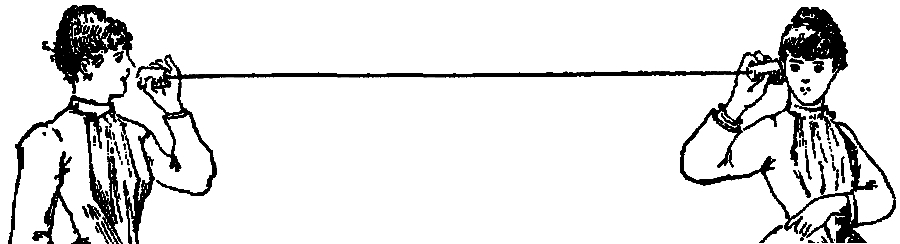
\includegraphics[width=0.6\textwidth]{../clipart/tincan.jpg}
        \end{figure}
    \end{frame}

    \begin{frame}
        \frametitle{Knowledge is difficult to comprehend}
        \begin{itemize}
        \item Knowledge is like feeling an elephant
        \item The human brain has a finite capacity working memory
        \item Many solutions cannot be grasped in their entirety
        \end{itemize}
        \begin{figure}[H]
            \centering
            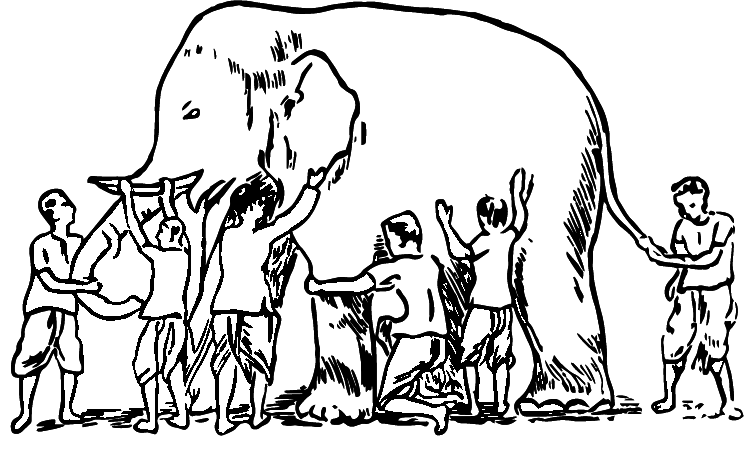
\includegraphics[width=0.5\textwidth]{../clipart/elephant.png}
        \end{figure}
    \end{frame}

    \begin{frame}
        \frametitle{Knowledge does not compose}
        \begin{itemize}
            \item Knowledge is not inherently compositional
            \item In order to make progress, we need programs to compose
            \item Impossible to do engineering by cobbling together spare parts
        \end{itemize}
        \begin{figure}[H]
            \centering
            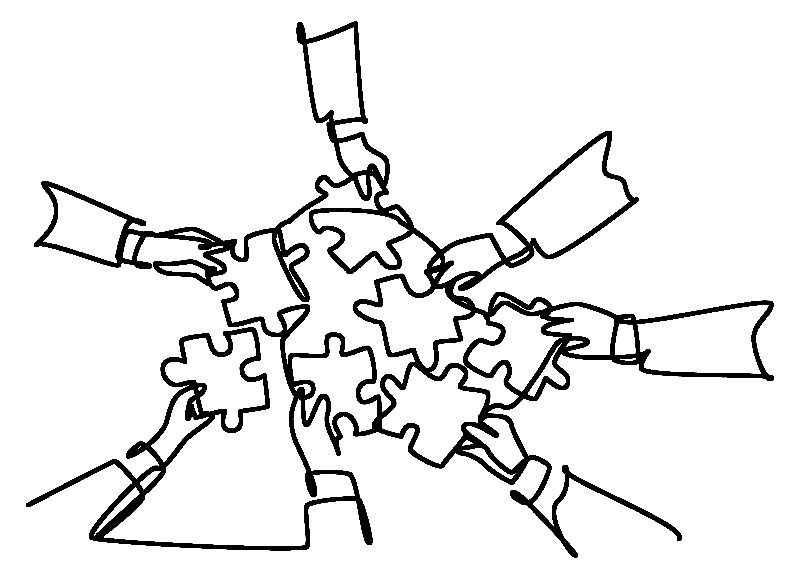
\includegraphics[width=0.5\textwidth]{../clipart/compositionality.jpeg}
        \end{figure}
    \end{frame}


    \begin{frame}
        \frametitle{Reason is a ladder to higher knowledge}
        \begin{itemize}
            \item To build understanding, we must have better tools
            \item Tools should complement human learning and reasoning
            \item Augmented intelligence through automated reasoning
            \item Reason is a tool to access higher order knowledge
        \end{itemize}
        \begin{figure}[H]
            \centering
            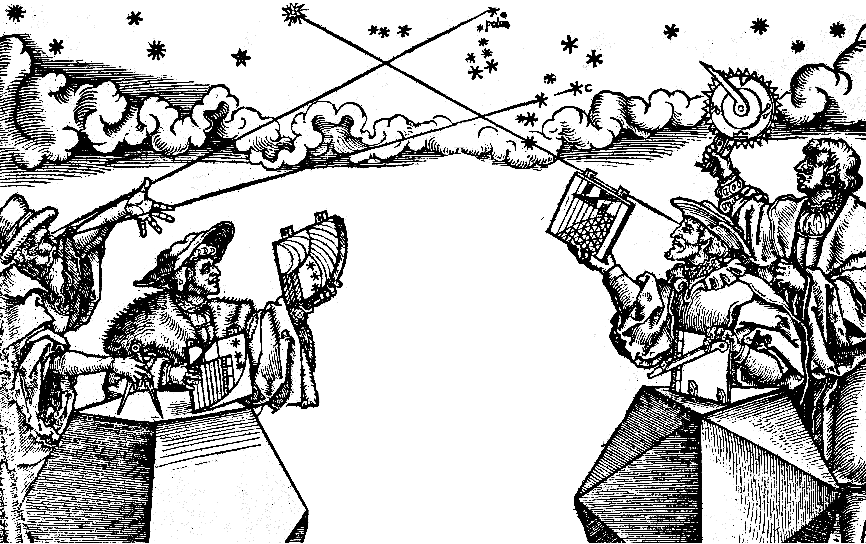
\includegraphics[width=0.5\textwidth]{../clipart/astronomers.png}
        \end{figure}
    \end{frame}

    \begin{frame}
        \frametitle{Reasoning from first principles}
        \begin{itemize}
            \item To learn programs, cannot imitate knowledge
            \item Too fragile, too many brittle assumptions
            \item Seek to understand process, not outcome
            \item Most software starts with pen and paper...
        \end{itemize}
        \begin{figure}[H]
            \centering

            \begin{prooftree}
                \bottomAlignProof
                \AxiomC{}
                \UnaryInfC{$a \sim a$}
                \noLine
                \UnaryInfC{}
                \noLine
                \UnaryInfC{\textit{Reflexivity}}
                \DisplayProof
                \hskip 1.5em
                \bottomAlignProof
                \AxiomC{$a \sim b$}
                \UnaryInfC{$b \sim a$}
                \noLine
                \UnaryInfC{}
                \noLine
                \UnaryInfC{\textit{Symmetry}}
                \DisplayProof
                \hskip 1.5em
                \bottomAlignProof
                \AxiomC{$a \sim b$}
                \AxiomC{$b \sim c$}
                \BinaryInfC{$a \sim c$}
                \noLine
                \UnaryInfC{}
                \noLine
                \UnaryInfC{\textit{Transitivity}}
                \DisplayProof
                \hskip 1.5em
                \bottomAlignProof
                \AxiomC{$a \sim b$}
                \UnaryInfC{$f(a) \sim f(b)$}
                \noLine
                \UnaryInfC{}
                \noLine
                \UnaryInfC{\textit{Congruence}}
            \end{prooftree}

        \end{figure}
    \end{frame}


    \begin{frame}
        \frametitle{Relations among probability distributions}
        \begin{itemize}
            \item Knowledge is accumulated across generations of research
            \item Patterns have specific names, e.g. ``Gaussian'', ``Dirichlet''...
            \item Can we infer these relations from first principles?
        \end{itemize}
        \begin{figure}[H]
            \centering
            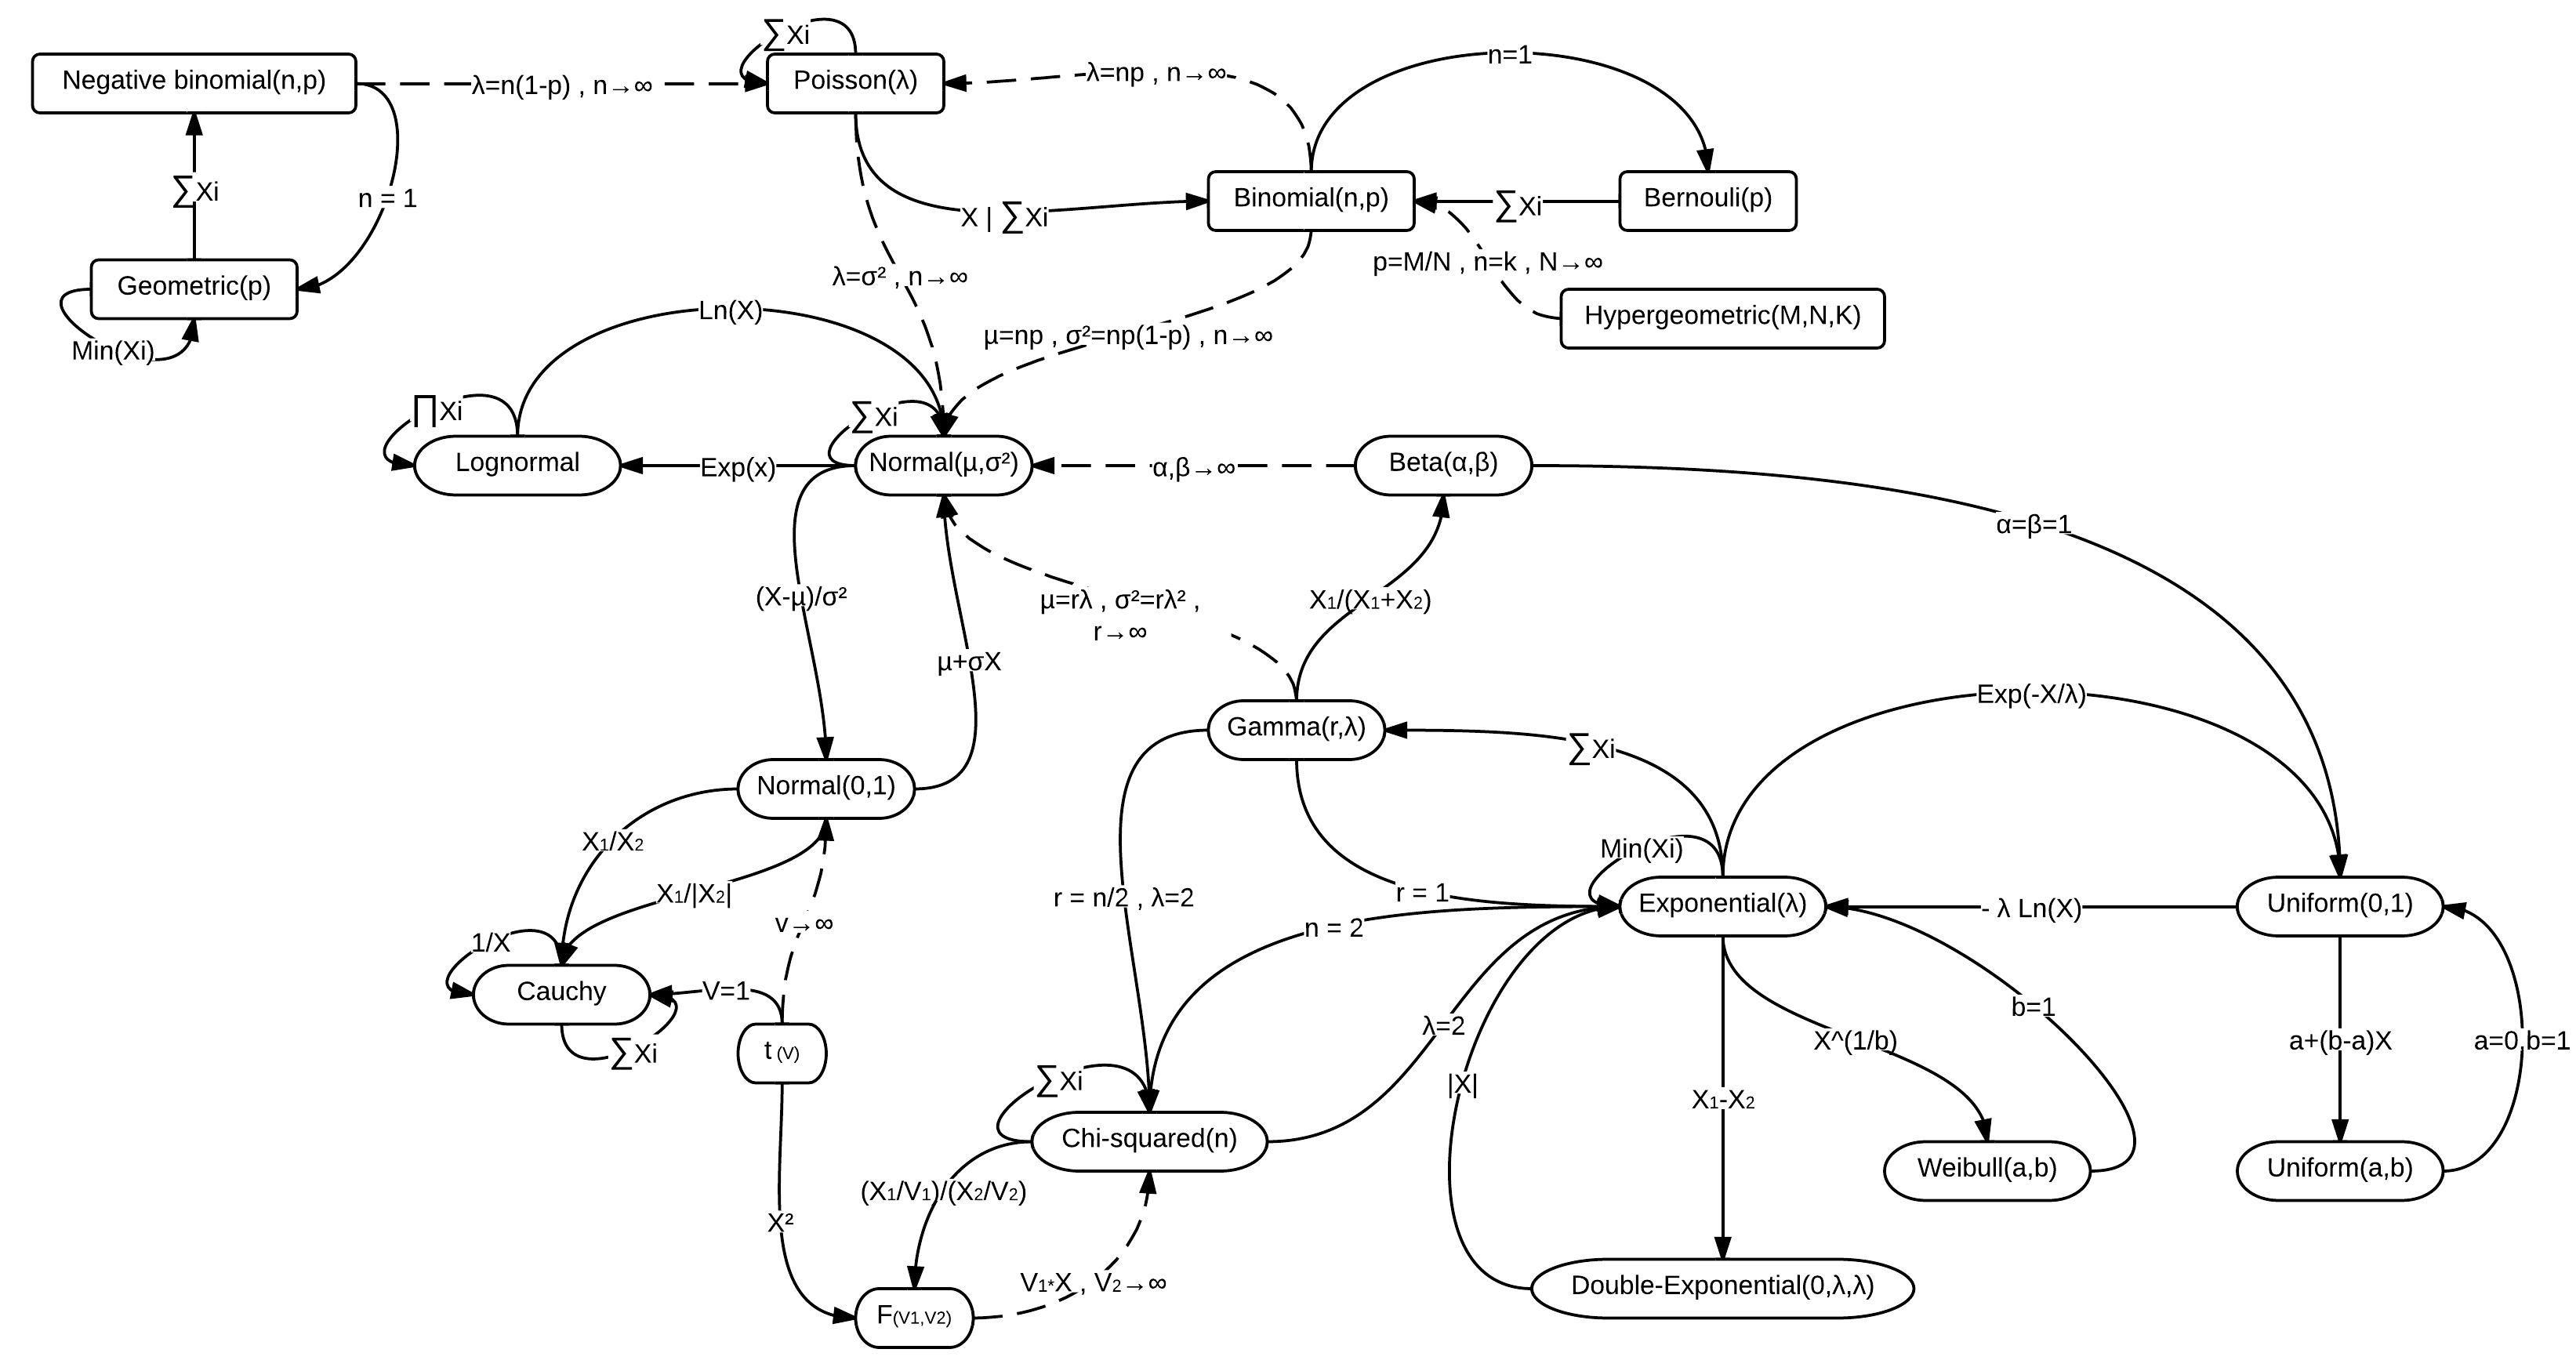
\includegraphics[width=0.7\textwidth]{../clipart/distribution_relations.jpeg}
        \end{figure}
    \end{frame}

\end{document}